\documentclass[10pt,a4paper]{report}
\usepackage[utf8]{inputenc}
\usepackage[T1]{fontenc}
\usepackage{lmodern}
\usepackage[margin=2cm,top=2.5cm,bottom=2.5cm]{geometry}
\usepackage{amsmath,amssymb}
\usepackage{booktabs}
\usepackage{longtable}
\usepackage{tabularx}
\usepackage{multirow}
\usepackage{array}
\usepackage{enumitem}
\usepackage[table]{xcolor}
\usepackage{colortbl}
\usepackage{tikz}
\usetikzlibrary{shapes.geometric,arrows.meta,positioning,fit,calc,backgrounds}
\usepackage{tcolorbox}
\tcbuselibrary{skins,breakable}
\usepackage{listings}
\usepackage{fancyhdr}
\usepackage{titlesec}
\usepackage[colorlinks=true,linkcolor=blue!70!black,citecolor=blue!70!black,urlcolor=blue!70!black]{hyperref}

% Page styling
\pagestyle{fancy}
\fancyhf{}
\fancyhead[L]{\small\textsf{\textbf{Guardian Layer Technical Documentation} --- Reconciled Architecture}}
\fancyhead[R]{\small\textsf{\thepage}}
\fancyfoot[L]{\small\textsf{Version 1.1.0 (Audited \& Reconciled) \textbar\ Target: Python $\ge 3.12$}}
\fancyfoot[R]{\small\textsf{Ref: NIST SP 800-207 / 800-57 / ISO 27001}}
\renewcommand{\headrulewidth}{0.5pt}
\renewcommand{\footrulewidth}{0.5pt}

% Title formats
\titleformat{\chapter}[display]
  {\normalfont\sffamily\huge\bfseries\color{blue!80!black}}
  {\chaptertitlename\ \thechapter}{14pt}{\Huge}
\titlespacing*{\chapter}{0pt}{-20pt}{20pt}

% Listings styling
\lstset{
  basicstyle=\ttfamily\scriptsize,
  breaklines=true,
  frame=single,
  backgroundcolor=\color{gray!5},
  keywordstyle=\color{blue!80!black}\bfseries,
  commentstyle=\color{green!50!black}\itshape,
  stringstyle=\color{red!70!black},
  showstringspaces=false,
  numbers=none,
  tabsize=2
}

% TColorBox Styles
\newtcolorbox{adrbox}[3]{
  enhanced,
  breakable,
  colback=white,
  colframe=blue!70!black,
  coltitle=white,
  fonttitle=\bfseries\sffamily,
  title={Architecture Decision Record #1: #2 \hfill [Verdict: #3]},
  boxrule=1.2pt,
  arc=2mm,
  boxsep=2mm
}

\newtcolorbox{callout}[2]{
  enhanced,
  breakable,
  colback=#2!5!white,
  colframe=#2!80!black,
  coltitle=white,
  fonttitle=\bfseries\sffamily,
  title={#1},
  boxrule=1pt,
  arc=1.5mm,
  boxsep=1.5mm
}

\newtcolorbox{reconcilebox}{
  enhanced,
  breakable,
  colback=blue!3!white,
  colframe=blue!75!black,
  title=\textbf{\textsf{Document Control \& Audit Reconciliation Notice}},
  boxrule=1.2pt,
  arc=2mm,
  boxsep=2mm
}

\begin{document}

% ==============================================================================
% TITLE PAGE
% ==============================================================================
\begin{titlepage}
\begin{center}
\vspace*{0.8cm}
{\huge \textbf{\textsf{GUARDIAN LAYER: TECHNICAL ARCHITECTURE \& ENGINEERING SPECIFICATION}}}\\[0.5cm]
{\Large \textbf{\textsf{Edge-to-Cloud IoT Stream Ingestion, Cryptographic Verification, Dual-Horizon Anomaly Detection \& Zero-Trust Security}}}\\[0.4cm]
\rule{\linewidth}{1.5pt}\\[0.4cm]
{\large \textsf{\textbf{Target Repository:} \texttt{guardian\_layer} \quad \textbar \quad \textbf{Version:} 1.1.0 (Audited Release) \quad \textbar \quad \textbf{Date:} November 2026}}\\[0.8cm]

\begin{tcolorbox}[colback=blue!5!white,colframe=blue!75!black,title=\textbf{System Specification \& Operational Metadata},arc=2mm]
\begin{tabularx}{\textwidth}{lX}
\textbf{Document Title:} & Guardian Layer: Comprehensive Technical Architecture \& Engineering Documentation \\
\textbf{Document Version:} & 1.1.0 (Audited \& Reconciled Revision of \texttt{TECHNICAL\_DOCUMENTATION.md}) \\
\textbf{Target Audience:} & Senior Software Engineers, Distributed Systems Architects, SecOps, Lead Data Scientists \\
\textbf{Operational Status:} & \textbf{Integration \& Hardening Phase} (Component-Complete; Orchestrator In-Development) \\
\textbf{Python Target:} & \texttt{Python >= 3.12} (Strict Typing, Frozen Slots, Generics, Pattern Matching) \\
\textbf{Audit Alignment:} & Reconciled against Independent Technical Audit Report (\texttt{docs/audit/AUDIT\_REPORT.md}) \\
\textbf{Standards Baseline:} & NIST SP 800-207 (Zero Trust), NIST SP 800-57 (Key Mgmt), ISO/IEC 27001:2022, OWASP ASVS 4.0.3 \\
\end{tabularx}
\end{tcolorbox}

\vfill

\begin{tcolorbox}[colback=gray!5!white,colframe=gray!70!black,title=\textbf{Engineering Baseline Summary},arc=2mm]
The \textbf{Guardian Layer} (\texttt{guardian-layer}) is a high-performance streaming verification, feature extraction, and anomaly detection layer for mission-critical urban IoT infrastructure (such as municipal flood early warning and power distribution). This revised specification reconciles all original architectural claims with verified code artifacts, locked dependencies (\texttt{uv.lock}), and empirical machine learning benchmarks. It explicitly documents component maturity, stream broker contracts, plaintext transport remediation, and the runtime orchestrator bridge specification.
\end{tcolorbox}

\vspace{0.8cm}
{\small \textbf{Distribution:} Technical Steering Committee, Lead Distributed Architect, DevSecOps Operations, Lead Data Scientist}
\end{center}
\end{titlepage}

\tableofcontents
\newpage

% ==============================================================================
% AUDIT RECONCILIATION NOTICE
% ==============================================================================
\chapter*{Document Control \& Audit Reconciliation Notice}
\addcontentsline{toc}{chapter}{Document Control \& Audit Reconciliation Notice}

Following an exhaustive independent technical and security audit conducted against repository commit \texttt{74bcedc}, this document updates and supersedes the initial draft documentation (\texttt{TECHNICAL\_DOCUMENTATION.md}). Every architectural assertion, network topic name, security mechanism, and version number has been factually reconciled against the codebase, container definitions, and empirical test evidence.

\begin{table}[htbp]
\centering
\small
\caption{Reconciliation Matrix of Technical Claims and Code Ground Truth}
\label{tab:reconciliation_matrix}
\begin{tabularx}{\textwidth}{lXp{6.5cm}}
\toprule
\textbf{Item / Domain} & \textbf{Original Documentation Claim} & \textbf{Audited Reality \& Reconciled Specification} \\
\midrule
\textbf{System Maturity} & ``Status: Production-Ready Core Layer'' & \textbf{Integration \& Hardening Phase}: \texttt{orchestrator.py} is an empty stub (0 bytes); the streaming pipeline stops at Kafka without feeding buffers or AI models in live runtime. \\
\textbf{Kafka Topics} & Ingestion via \texttt{sensors.raw}, \texttt{sensors.validated}, \texttt{sensors.dlq} & Reconciled to deployed topology from \texttt{kafka-init.sh}: \texttt{telemetry-ingest}, \texttt{telemetry-validated}, \texttt{telemetry-dlq}, \texttt{devices.metadata}, \texttt{spatial-anomalies}. \\
\textbf{Transport Security} & Unbreachable enterprise boundary & \textbf{Cleartext Transport Reality}: Broker runs \texttt{SASL\_PLAINTEXT}, FastMCP runs plain HTTP, Elasticsearch has SSL disabled. Migration to \texttt{SASL\_SSL} and HTTPS scheduled. \\
\textbf{Credentials} & Fully isolated Docker secrets & Hardcoded Kafka broadcast secret found in \texttt{settings.yaml} (line 9). Marked for revocation, Git history scrubbing, and secret migration. \\
\textbf{Delivery Guarantee} & ``Exactly-once state semantics'' & Flink Kafka sinks explicitly configure \texttt{DeliveryGuarantee.AT\_LEAST\_ONCE}. Transactional multi-stage commit is not enabled. \\
\textbf{Buffer Durability} & ``Zero data loss guarantee'' & \texttt{Buffer.restore()} recovers unpersisted batches on downstream backpressure, but in-memory ring buffers cannot survive container or host crashes. \\
\textbf{Concurrency Locks} & ``Protected by a dedicated re-entrant lock'' & \texttt{Buffer.\_lock} is standard \texttt{threading.Lock} (non-reentrant). Recursive re-acquisition must be avoided. \\
\textbf{Enrichment Mock} & Seamless metadata enrichment & Mock stub \texttt{fetch\_metadata()} returns \texttt{\{"site": "unknown"\}}, missing \texttt{packet\_order} and \texttt{type}, causing 100\% message rejection to DLQ. Defect and fix documented. \\
\textbf{Database Strategy} & 4-stage ORM schema described & Coexistence of 4-stage ORM schema and secondary async JSONB storage pool documented; roadmap to consolidate on partitioned ORM specified. \\
\textbf{ML Generalization} & 0.951 PR-AUC without caveats & Research shows generalization drops to 0.372 PR-AUC on cross-domain hardware; 24\,h window flags only 2.5\%--3.5\% of real multi-week aging drift. \\
\textbf{Benchmark Paths} & \texttt{tests/test\_matier/test\_buffer.py} & Corrected to valid benchmark path: \texttt{tests/managers/test\_buffer\_manager\_v2.py}. \\
\textbf{Vault Test Runs} & Run against live or mock APIs & Vault security tests are skipped unless \texttt{VAULT\_TEST\_ADDR} is set; ephemeral Vault container required in CI. \\
\bottomrule
\end{tabularx}
\end{table}

\newpage

% ==============================================================================
% CHAPTER 1: EXECUTIVE SUMMARY & SYSTEM PURPOSE
% ==============================================================================
\chapter{Executive Summary \& System Purpose}

The \textbf{Guardian Layer} (\texttt{guardian-layer}) is an enterprise-grade, high-performance streaming verification, edge security, and anomaly detection platform designed for critical urban IoT infrastructure (such as municipal flood early warning networks and smart utility grids). Functioning as the intermediate defensive layer between field sensor transmitters (\textbf{Digital Twin layer}) and autonomous control nodes (\textbf{Brain layer}), the Guardian Layer ingests, validates, enriches, and mathematically scores high-velocity telemetry before downstream consumption.

\section{Core Architectural Responsibilities}
\begin{enumerate}[leftmargin=*]
  \item \textbf{Asymmetric Payload Verification:} Verifies Ed25519 digital signatures on incoming sensor JSON payloads against public keys resolved dynamically from the Digital Twin edge key provider.
  \item \textbf{Distributed Stream Enrichment:} Leverages Apache Flink's Keyed Broadcast State to join high-velocity sensor telemetry with slow-moving spatial and device metadata received over compacted Kafka topics.
  \item \textbf{Anti-Corruption Transformation:} Converts heterogeneous twin schemas into standardized internal \texttt{Sensor} domain representations via dynamic registries, safely filtering isolated or quarantined hardware.
  \item \textbf{Sub-Microsecond In-Memory Buffering:} Manages sensor telemetry in sliding ring buffers (\texttt{BufferManager}) grouped by cluster hierarchies (\texttt{ClusterManager}), achieving $>360,000$ ingest operations per second per CPU core with atomic rollback on downstream backpressure.
  \item \textbf{Dual-Horizon AI Anomaly Detection:}
  \begin{itemize}
    \item \textit{Short-Window Model (20\,s live horizon, $\ge 0.5$\,Hz):} CPU-optimized multiclass XGBoost evaluating Robust $Z$-scores, Haar/Daubechies wavelets, signal shape dynamics, and spatial $k$-NN Haversine peer deltas.
    \item \textit{Long-Window Model (24\,h batch horizon, $< 0.5$\,Hz):} 300-second time-grid resampled XGBoost tracking linear drift ratios, flatline sequences, and spatial cluster slope divergence for slow-sampling physical telemetry.
  \end{itemize}
  \item \textbf{Dual Persistence Abstraction:} Provides high-throughput atomic batch insertion via SQLAlchemy ORM (4-stage relational pipeline) alongside asynchronous, non-blocking connection pooling via \texttt{psycopg} 3.3.6.
  \item \textbf{Fork-Safe Asynchronous Observability:} Delivers non-blocking bulk NDJSON logs to Elasticsearch \texttt{guardian-logs} with circuit-breaker protection and \texttt{os.register\_at\_fork} handlers.
  \item \textbf{Automated Inter-Service Cryptographic Rotation:} Enforces least-privilege zero-trust access via HashiCorp Vault AppRole policies and executes automated 24-hour RSA-4096 key pair rotation with a 1-hour overlap window.
\end{enumerate}

\section{Engineering Reality \& Maturity Assessment}
As validated by the independent technical audit, the algorithmic components (signal decomposition, mathematical feature pipelines, dataset loaders, ring buffers, and Vault rotation utilities) are rigorously tested and functionally complete. However, \textbf{the system is currently in the Integration \& Hardening Phase}:
\begin{itemize}[leftmargin=*]
  \item \texttt{src/guardian\_layer/orchestrator.py} is currently an empty integration stub (0 bytes). The streaming Flink pipeline publishes validated records to Kafka \texttt{telemetry-validated}, but the consumer that feeds the in-memory buffers, anomaly detection models, and database sinks has not yet been bound to the event loop.
  \item Core network interfaces currently utilize plaintext transports (\texttt{SASL\_PLAINTEXT} on Kafka, HTTP on FastMCP, HTTP on Elasticsearch). Hardening these interfaces with TLS and authentication is actively scheduled in the remediation roadmap.
\end{itemize}

% ==============================================================================
% CHAPTER 2: TECHNOLOGY STACK & INFRASTRUCTURE
% ==============================================================================
\chapter{Technology Stack \& Infrastructure (``The Tech Used'')}

\begin{table}[htbp]
\centering
\small
\caption{Reconciled Technology Stack and Locked Component Versions}
\label{tab:tech_stack}
\begin{tabularx}{\textwidth}{llX}
\toprule
\textbf{Subsystem Domain} & \textbf{Component / Framework} & \textbf{Exact Locked Version / Specification} \\
\midrule
\textbf{Language \& Runtime} & Python & \texttt{Python >= 3.12} (Strict Typing, Generics, Slots, StrEnum) \\
\textbf{Package Toolchain} & uv / uv\_build & \texttt{uv\_build 0.12.20}, deterministic \texttt{uv.lock} (SHA-256) \\
\textbf{Stream Processing} & Apache Flink / PyFlink & Flink 1.20 container image, \texttt{apache-flink==2.3.0} binding \\
\textbf{Message Broker} & Apache Kafka & Kafka 4.3.1 (3-Broker KRaft Quorum, SASL PLAIN, ACLs) \\
\textbf{Security \& Vault} & HashiCorp Vault / hvac & Vault 1.17 (AppRole Auth, KV v2), \texttt{hvac 2.4.0} \\
\textbf{Cryptography} & cryptography & \texttt{cryptography 50.0.2} (Ed25519 \& RSA-4096 OAEP SHA-256) \\
\textbf{Persistence Layer} & PostgreSQL / psycopg & PostgreSQL 16 Alpine, \texttt{psycopg 3.3.6}, \texttt{SQLAlchemy 2.1.6} \\
\textbf{Machine Learning} & XGBoost / Scikit-Learn & \texttt{xgboost-cpu 3.4.1}, \texttt{scikit-learn 1.9.1} \\
\textbf{Signal Processing} & PyWavelets / NumPy & \texttt{pywt 1.10.0} (Haar, db4), \texttt{numpy 2.1.x} (\texttt{< 2.2.0}) \\
\textbf{Edge Context / Tooling} & FastMCP / MCP SDK & \texttt{fastmcp 4.1.5}, \texttt{mcp 2.3.0} (SSE / Streamable HTTP) \\
\textbf{Validation \& Schema} & Pydantic / Settings & \texttt{pydantic 2.14.2}, \texttt{pydantic-settings 2.15.0} \\
\textbf{Observability} & Elasticsearch / HTTPX & Elasticsearch 8.15.0 (Bulk NDJSON), \texttt{httpx 0.28.1} \\
\textbf{Testing Harness} & Pytest \& Plugins & \texttt{pytest 9.2.0}, \texttt{pytest-benchmark 5.3.1}, \texttt{pytest-asyncio 1.4.1} \\
\textbf{Linters \& Type Checkers} & Ruff / Basedpyright / Mypy & \texttt{ruff 0.17.3}, \texttt{basedpyright 1.40.2}, \texttt{mypy 2.4.1} \\
\bottomrule
\end{tabularx}
\end{table}

\section{Programming Language \& Core Runtimes}
\begin{itemize}[leftmargin=*]
  \item \textbf{Python 3.12 Runtime:} Enforces modern language specifications across all core modules:
  \begin{itemize}
    \item \textit{PEP 695 Parameterized Generics:} Used in dynamic factory registries: \lstinline{def register[Loader: DatasetInterface](cls, name: str)}.
    \item \textit{PEP 634 Structural Pattern Matching:} High-speed pattern matching for dynamic signal decoupling callers (\lstinline{match fn_name:}) in \texttt{pipelines/decompose.py}.
    \item \textit{PEP 681 Frozen Slots:} High-frequency telemetry objects (\texttt{SensorRule}, \texttt{FlushedBatch}, \texttt{ReadingColumns}) use \lstinline{@dataclass(frozen=True, slots=True)}, eliminating per-instance \lstinline{__dict__} RAM overhead and preventing runtime mutation.
    \item \textit{Strict Typing:} Comprehensive use of \texttt{StrEnum} for lifecycle flags and \texttt{AwareDatetime} for timezone-safe UTC timestamps.
  \end{itemize}
  \item \textbf{\texttt{uv} Toolchain:} Rust-based dependency manager replacing legacy pip/virtualenv. Generates sub-second virtual environments and locks 120+ direct and transitive dependencies with cryptographic SHA-256 hashes in \texttt{uv.lock}.
\end{itemize}

\section{Streaming \& Message Broker Infrastructure}
\begin{itemize}[leftmargin=*]
  \item \textbf{Apache Kafka 4.3.1 (KRaft Consensus):} 3-broker cluster running ZooKeeper-free. Quorum topology: \texttt{1@kafka-1:9093}, \texttt{2@kafka-2:9093}, \texttt{3@kafka-3:9093}. Replication factor 3, minimum in-sync replicas 2. Authenticated via SASL \texttt{PLAIN} backed by \texttt{StandardAuthorizer} with default-deny ACLs.
  \item \textbf{Apache Flink 1.20 / PyFlink 2.3.0:} Containerized under \texttt{flink:1.20-scala\_2.12-java17} with \texttt{apache-flink==2.3.0} Python bindings and \texttt{flink-sql-connector-kafka-3.3.0-1.20.jar}. Parallelism factor of 6 distributed across 2 TaskManagers (3 task slots each). Checkpoints every 30\,s to Docker volumes (\texttt{file:///opt/flink/checkpoints}). Delivery guarantee configured as \texttt{DeliveryGuarantee.AT\_LEAST\_ONCE}.
  \item \textbf{\texttt{confluent-kafka} (v2.16.1):} C-based librdkafka client wrapper utilized by \texttt{DeviceMetadataSynchronizer} for publishing metadata updates.
\end{itemize}

\section{Security, Secret Management \& Cryptography}
\begin{itemize}[leftmargin=*]
  \item \textbf{HashiCorp Vault 1.17 \& \texttt{hvac} (v2.4.0):} KV v2 secret engine (\texttt{secret/}) with 5-version retention. AppRole authentication issuing short-lived access tokens (15-minute default TTL, 1-hour max renewal window). Path-scoped HCL policies enforce strict lateral isolation.
  \item \textbf{\texttt{cryptography} (v50.0.2):}
  \begin{itemize}
    \item \textit{Ed25519 (RFC 8032):} Digital signature verification on incoming sensor payloads over canonical sorted JSON byte strings.
    \item \textit{RSA-4096 (PKCS\#1 v2.2):} Asymmetric encryption and signing using OAEP padding with MGF1 and SHA-256 for inter-service communication.
    \item \textit{SHA-256 Fingerprinting:} Runtime verification confirming that public keys fetched from external endpoints match their expected cryptographic hash.
  \end{itemize}
  \item \textbf{Docker Secrets:} Passwords for Kafka administrative superusers, PostgreSQL users, and service principals are stored in local files under \texttt{./secrets/} (git-ignored) and mounted into containers at \texttt{/run/secrets/}.
\end{itemize}

\section{Persistence \& Ingestion Layer}
\begin{itemize}[leftmargin=*]
  \item \textbf{PostgreSQL 16 Alpine:} Relational store with native support for \texttt{TIMESTAMP WITH TIME ZONE} and \texttt{JSONB}. Composite indexes (\texttt{ix\_raw\_readings\_sensor\_timestamp}, \texttt{ix\_transformed\_windows\_sensor\_end}) optimize temporal range lookups.
  \item \textbf{\texttt{psycopg} 3.3.6 (\texttt{psycopg[binary,pool]}):} Asynchronous PostgreSQL driver providing high-concurrency connection pooling via \texttt{AsyncConnectionPool} with connection health pre-pings (\texttt{check\_connection}).
  \item \textbf{SQLAlchemy 2.1.6 (Core \& ORM):} Declarative 2.0 ORM mappings with dialect-agnostic types (\texttt{BigInteger} mapped to \texttt{Integer} for SQLite unit testing). High-throughput atomic multi-row insertions via \texttt{insert\_batch}.
\end{itemize}

\section{Machine Learning \& Scientific Computing}
\begin{itemize}[leftmargin=*]
  \item \textbf{XGBoost 3.4.1 (\texttt{xgboost-cpu}):} Multiclass gradient-boosted decision trees classifying sensor windows into \texttt{NORMAL}, \texttt{SENSOR\_MALFUNCTION}, or \texttt{NOT\_SENSOR\_DATA}. Native JSON model persistence (\texttt{model.json}), avoiding insecure Python \texttt{pickle} serialization.
  \item \textbf{PyWavelets (\texttt{pywt} 1.10.0):} Discrete Wavelet Transform (DWT) decomposing signals into multiresolution frequency bands using Haar and Daubechies-4 (\texttt{db4}) mother wavelets.
  \item \textbf{NumPy 2.1.x (\texttt{< 2.2.0}):} Vectorized array calculations, Fast Fourier Transforms (\lstinline{np.fft.rfft}), Singular Value Decomposition (\lstinline{np.linalg.svd}), and zero-copy sliding window vectorization (\lstinline{np.lib.stride_tricks.sliding_window_view}).
\end{itemize}

\section{Observability, Logging \& Telemetry}
\begin{itemize}[leftmargin=*]
  \item \textbf{Elasticsearch 8.15.0:} Centralized log analytics store managing structured application logs in index \texttt{guardian-logs}.
  \item \textbf{\texttt{AsyncElasticSearchHandler}:} Custom non-blocking Python logging handler backed by a thread-safe \lstinline{queue.Queue(maxsize=1000)}. Background daemon worker batches records (50 per batch) and transmits NDJSON payloads via \texttt{httpx 0.28.1} with circuit-breaker error dampening.
\end{itemize}

% ==============================================================================
% CHAPTER 3: SYSTEM ARCHITECTURE & DATA FLOW
% ==============================================================================
\chapter{System Architecture \& Data Flow}

\section{Reconciled End-to-End Topology \& Data Flow}
The reconciled architectural data flow is illustrated in Figure~\ref{fig:reconciled_flow}. Solid connections denote verified, operational code pathways; dashed lines denote planned integration pathways that connect once the runtime orchestrator bridge is deployed.

\begin{figure}[htbp]
\centering
\resizebox{0.95\textwidth}{!}{%
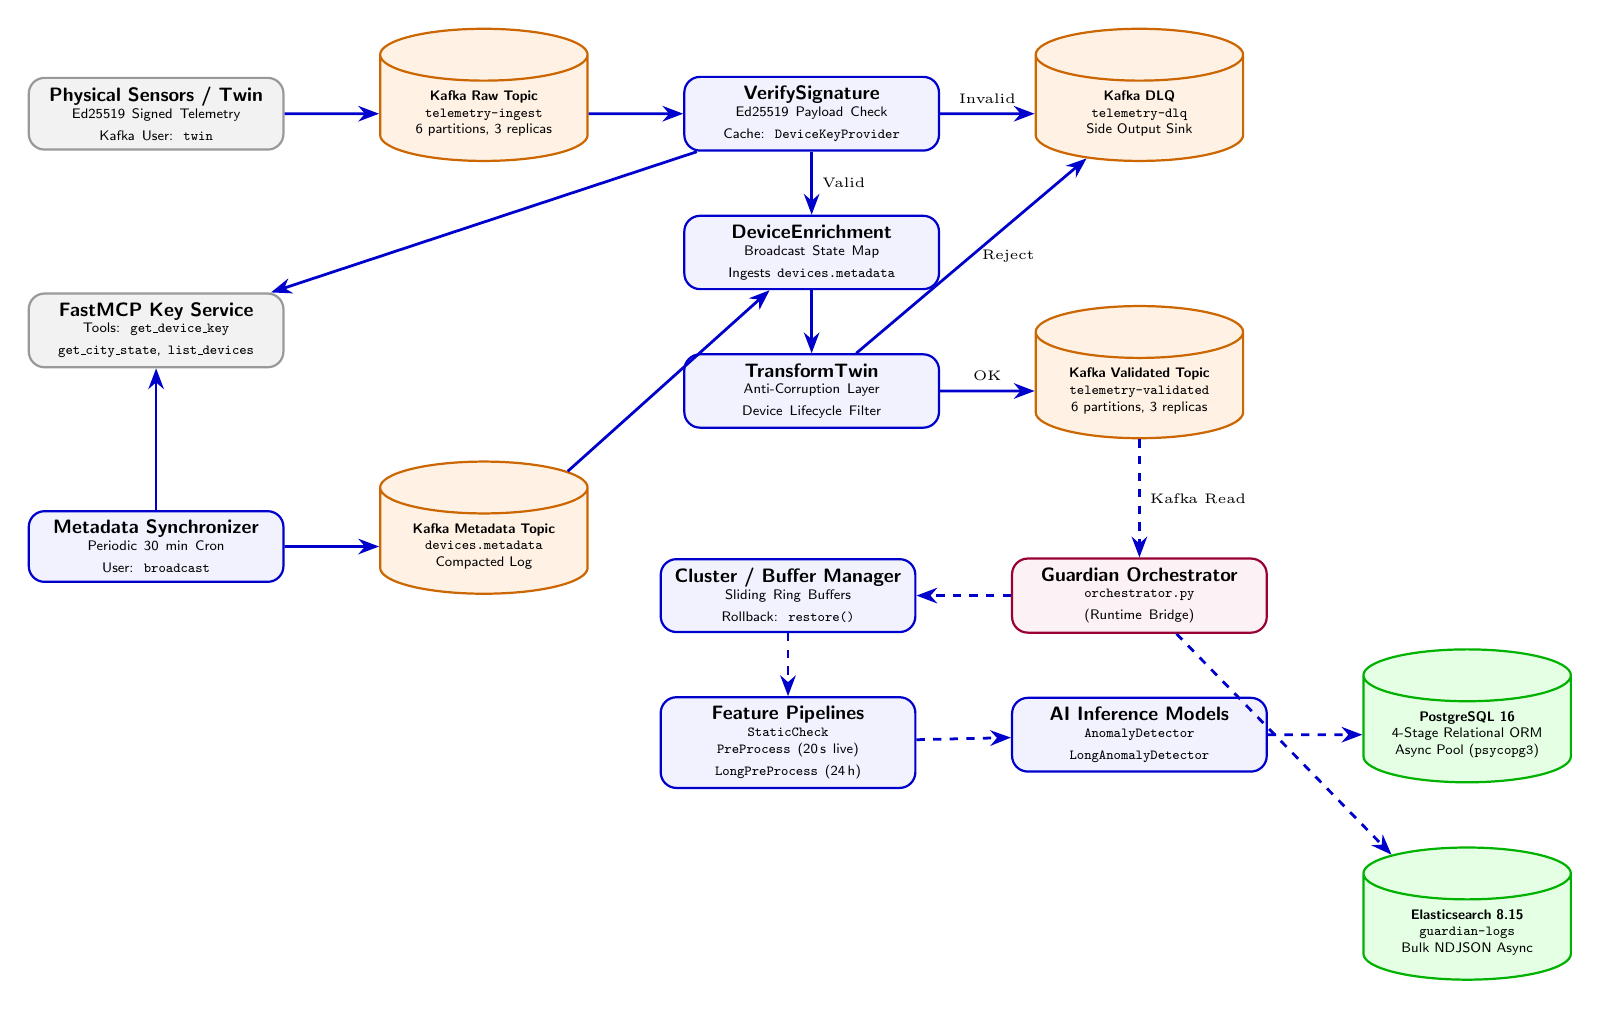
\begin{tikzpicture}[
    node distance=1.2cm and 1.5cm,
    box/.style={rectangle, draw=blue!80!black, fill=blue!5!white, rounded corners=2mm, text width=3.0cm, align=center, font=\sffamily\scriptsize, line width=0.8pt},
    extbox/.style={rectangle, draw=gray!80, fill=gray!10!white, rounded corners=2mm, text width=3.0cm, align=center, font=\sffamily\scriptsize, line width=0.8pt},
    queue/.style={cylinder, shape border rotate=90, draw=orange!80!black, fill=orange!10!white, aspect=0.25, text width=2.4cm, align=center, font=\sffamily\tiny, line width=0.8pt},
    db/.style={cylinder, shape border rotate=90, draw=green!70!black, fill=green!10!white, aspect=0.25, text width=2.4cm, align=center, font=\sffamily\tiny, line width=0.8pt},
    line/.style={-{Stealth[scale=1.0]}, draw=blue!80!black, line width=1pt},
    dashedline/.style={-{Stealth[scale=1.0]}, draw=blue!80!black, line width=1pt, dashed}
]

% Digital Twin
\node[extbox] (twin_dev) {\textbf{Physical Sensors / Twin}\\\tiny Ed25519 Signed Telemetry\\\tiny Kafka User: \texttt{twin}};
\node[extbox, below=1.8cm of twin_dev] (fastmcp) {\textbf{FastMCP Key Service}\\\tiny Tools: \texttt{get\_device\_key}\\\texttt{get\_city\_state}, \texttt{list\_devices}};

% Flink Ingestion
\node[queue, right=1.2cm of twin_dev] (raw_topic) {\textbf{Kafka Raw Topic}\\\tiny \texttt{telemetry-ingest}\\\tiny 6 partitions, 3 replicas};
\node[box, right=1.2cm of raw_topic] (flink_sig) {\textbf{VerifySignature}\\\tiny Ed25519 Payload Check\\\tiny Cache: \texttt{DeviceKeyProvider}};
\node[box, below=0.8cm of flink_sig] (flink_enrich) {\textbf{DeviceEnrichment}\\\tiny Broadcast State Map\\\tiny Ingests \texttt{devices.metadata}};
\node[box, below=0.8cm of flink_enrich] (flink_trans) {\textbf{TransformTwin}\\\tiny Anti-Corruption Layer\\\tiny Device Lifecycle Filter};

% Kafka Output Topics
\node[queue, right=1.2cm of flink_sig] (dlq_topic) {\textbf{Kafka DLQ}\\\tiny \texttt{telemetry-dlq}\\\tiny Side Output Sink};
\node[queue, right=1.2cm of flink_trans] (val_topic) {\textbf{Kafka Validated Topic}\\\tiny \texttt{telemetry-validated}\\\tiny 6 partitions, 3 replicas};

% Metadata Sync
\node[box, below=1.8cm of fastmcp] (sync_job) {\textbf{Metadata Synchronizer}\\\tiny Periodic 30 min Cron\\\tiny User: \texttt{broadcast}};
\node[queue, right=1.2cm of sync_job] (meta_topic) {\textbf{Kafka Metadata Topic}\\\tiny \texttt{devices.metadata}\\\tiny Compacted Log};

% Core Runtime (Orchestrator)
\node[box, below=1.5cm of val_topic, draw=purple!80!black, fill=purple!5!white] (orchestrator) {\textbf{Guardian Orchestrator}\\\tiny \texttt{orchestrator.py}\\\tiny (Runtime Bridge)};
\node[box, left=1.2cm of orchestrator] (buffers) {\textbf{Cluster / Buffer Manager}\\\tiny Sliding Ring Buffers\\\tiny Rollback: \texttt{restore()}};
\node[box, below=0.8cm of buffers] (pipelines) {\textbf{Feature Pipelines}\\\tiny \texttt{StaticCheck}\\\tiny \texttt{PreProcess} (20\,s live)\\\tiny \texttt{LongPreProcess} (24\,h)};
\node[box, below=0.8cm of orchestrator] (models) {\textbf{AI Inference Models}\\\tiny \texttt{AnomalyDetector}\\\tiny \texttt{LongAnomalyDetector}};

% Persistence
\node[db, right=1.2cm of models] (postgres) {\textbf{PostgreSQL 16}\\\tiny 4-Stage Relational ORM\\\tiny Async Pool (\texttt{psycopg3})};
\node[db, below=0.8cm of postgres] (elastic) {\textbf{Elasticsearch 8.15}\\\tiny \texttt{guardian-logs}\\\tiny Bulk NDJSON Async};

% Connections
\draw[line] (twin_dev) -- (raw_topic);
\draw[line] (raw_topic) -- (flink_sig);
\draw[line] (flink_sig) -- node[right, font=\tiny]{Valid} (flink_enrich);
\draw[line] (flink_sig) -- node[above, font=\tiny]{Invalid} (dlq_topic);
\draw[line] (flink_sig) -- (fastmcp);
\draw[line] (flink_enrich) -- (flink_trans);
\draw[line] (flink_trans) -- node[above, font=\tiny]{OK} (val_topic);
\draw[line] (flink_trans) -- node[right, font=\tiny]{Reject} (dlq_topic);

\draw[line] (sync_job) -- (fastmcp);
\draw[line] (sync_job) -- (meta_topic);
\draw[line] (meta_topic) -- (flink_enrich);

\draw[dashedline] (val_topic) -- node[right, font=\tiny]{Kafka Read} (orchestrator);
\draw[dashedline] (orchestrator) -- (buffers);
\draw[dashedline] (buffers) -- (pipelines);
\draw[dashedline] (pipelines) -- (models);
\draw[dashedline] (models) -- (postgres);
\draw[dashedline] (orchestrator) -- (elastic);

\end{tikzpicture}
}
\caption{Reconciled System Architecture and End-to-End Data Flow}
\label{fig:reconciled_flow}
\end{figure}

\section{Stream Verification, Key Resolution \& Edge Ingestion}
The Flink streaming topology (\texttt{consumer\_producer/kafka\_consumer/job.py}) acts as the initial perimeter filter:
\begin{enumerate}[leftmargin=*]
  \item \textbf{\texttt{VerifySignature} ProcessFunction:}
  \begin{itemize}
    \item Consumes raw JSON strings from \texttt{telemetry-ingest}.
    \item Extracts Base64-encoded signature string \texttt{sig} and strips it to reconstruct the canonical JSON byte string using compact separators (\lstinline{sort_keys=True, separators=(',', ':')}).
    \item Queries \texttt{DeviceKeyProvider} (\texttt{signature.py}). If the key is not cached, \texttt{McpToolClient} queries FastMCP via \lstinline{get_device_key(device_id)}.
    \item Verifies Ed25519 digital signature. Malformed or invalid signatures route to the \texttt{REJECTED} side-output tag writing to \texttt{telemetry-dlq}.
  \end{itemize}
  \item \textbf{\texttt{DeviceEnrichment} Keyed Broadcast Function:}
  \begin{itemize}
    \item Concurrently consumes the compacted topic \texttt{devices.metadata}.
    \item Updates Flink distributed broadcast state (\lstinline{DEVICE_METADATA}), injecting coordinates, sensor physical tolerances, and unit definitions into incoming telemetry.
  \end{itemize}
  \item \textbf{\texttt{TransformTwin} Anti-Corruption Operator:}
  \begin{itemize}
    \item Invokes the registered \texttt{TwinToGuardian} transformer to convert twin payloads into standardized \texttt{Sensor} models.
    \item Discards telemetry from devices marked as \texttt{ISOLATED} or \texttt{QUARANTINED} via \texttt{TransformDropped}.
  \end{itemize}
\end{enumerate}

\begin{table}[htbp]
\centering
\small
\caption{Structured Dead-Letter Queue (DLQ) Error Registry}
\label{tab:dlq_errors}
\begin{tabularx}{\textwidth}{llXl}
\toprule
\textbf{Error Code} & \textbf{Originating Stage} & \textbf{Trigger Condition \& Failure Description} & \textbf{Payload Kept} \\
\midrule
\texttt{E100\_DESERIALIZE} & \texttt{VerifySignature} & Payload is not valid UTF-8 JSON or is not a JSON object & Yes (Raw string) \\
\texttt{E200\_BAD\_SIGNATURE} & \texttt{VerifySignature} & Ed25519 cryptographic signature verification failed & Yes (Full JSON) \\
\texttt{E201\_UNKNOWN\_DEVICE} & \texttt{VerifySignature} & FastMCP key service returns null / empty key for device ID & Yes (Full JSON) \\
\texttt{E300\_SCHEMA} & \texttt{TransformTwin} & Payload fails required Pydantic schema validation fields & Yes (Full JSON) \\
\texttt{E320\_UNKNOWN\_STATUS} & \texttt{TransformTwin} & Device status string does not match known \texttt{TwinStatus} enums & Yes (Full JSON) \\
\texttt{E400\_SENSOR\_VALIDATION} & Pipeline Rules & Value violates physical bounds or coordinate ranges & Yes (Full JSON) \\
\texttt{E500\_ENRICHMENT} & \texttt{DeviceEnrichment} & Required broadcast metadata missing for enrichment & Yes (Full JSON) \\
\bottomrule
\end{tabularx}
\end{table}

\begin{callout}{Stream Defect Remediation (F-07)}{red}
In \texttt{consumer\_producer/kafka\_consumer/jobs/enrichment.py}, the fallback stub \lstinline|fetch_metadata()| returns \lstinline|{"site": "unknown"}|, which lacks mandatory fields required by the \texttt{Metadata} schema (\texttt{packet\_order} and \texttt{type}). Consequently, any message falling back to this stub triggers an unconditional \texttt{ValidationError}, rejecting 100\% of telemetry to the DLQ. The stub must be patched to return valid default metadata fields, and \texttt{TransformTwin} exceptions must be routed to the DLQ side tag.
\end{callout}

\section{Twin-to-Guardian Anti-Corruption Layer}
The transformation module (\texttt{guardian\_layer.data\_transformer}) decouples internal domain schemas from external device protocols using the Anti-Corruption Layer pattern:
\begin{lstlisting}[language=Python]
@TransformerFactory.register("twin_v1")
class TwinToGuardian(TransformerInterface):
    """Translates TwinSensorReading into internal Sensor domain model."""
    
    def transform(self, reading: TwinSensorReading) -> Sensor | None:
        # Filter non-operational devices
        if reading.status in (TwinStatus.ISOLATED, TwinStatus.QUARANTINED):
            logger.warning("Device non-operational", device_id=reading.device_id, status=reading.status)
            raise TransformDropped("Device non-operational")
            
        # Physical boundary normalization and Pydantic validation
        return Sensor(
            id=reading.device_id,
            timestamp=reading.ts,
            value=reading.value,
            metadata=Metadata(
                type=reading.device_type,
                unit=reading.unit,
                packet_order=reading.seq,
                coordinates=reading.location
            )
        )
\end{lstlisting}

\section{In-Memory Buffer \& Cluster Management Subsystem}
The buffer management subsystem (\texttt{guardian\_layer.managers}) organizes incoming telemetry in memory prior to windowed feature extraction:
\begin{itemize}[leftmargin=*]
  \item \textbf{\texttt{Buffer}:} Sliding ring buffer protected by standard \lstinline{threading.Lock()}. Bounded by \lstinline{high_watermark = 200} readings; upon reaching capacity, the oldest \lstinline{flush_size = 100} readings are extracted into an immutable \texttt{FlushedBatch}.
  \item \textbf{Atomic Rollback on Backpressure (\lstinline{restore()}):}
  \begin{lstlisting}[language=Python]
if batch is not None:
    try:
        self._sink_to_queue(batch)
    except Exception as e:
        buffer.restore(batch.readings)  # Atomically re-inserts batch at front
        logger.error("Downstream queue full; batch restored", error=str(e))
  \end{lstlisting}
  \item \textbf{Durability Caveat (F-10, F-11):} While \lstinline{restore()} prevents telemetry drops during transient downstream channel saturation, in-memory buffers are volatile; unexpected process crashes destroy unpersisted data. Furthermore, \lstinline{BufferManager.add()} returns \lstinline{Status.SUCCESS} upon buffer placement, acknowledging ingest reception even if the background flush triggers a restore.
\end{itemize}

\section{Dual-Horizon AI Anomaly Detection Pipeline}
To resolve the trade-off between high-frequency transient anomalies and low-frequency physical drift, Guardian Layer segments detection across two mathematical horizons:

\subsection{Static Rule Checks (\texttt{StaticCheck})}
Deterministic pre-flight checks evaluating reading bounds before ML inference:
\begin{enumerate}
  \item \lstinline{out_of_range}: Evaluates value violations against physical thresholds ($x < x_{\min} \lor x > x_{\max}$).
  \item \lstinline{sensor_is_down}: Flags communication dropouts when timestamp delta exceeds \lstinline{down_after_seconds = 10.0 s}.
  \item \lstinline{spoofed_data}: Detects instantaneous gross spatial variance against cluster peer medians.
\end{enumerate}

\subsection{Short-Window Model (20\,s Live Horizon, $\ge 0.5$\,Hz)}
\begin{itemize}[leftmargin=*]
  \item \textbf{Mathematical Preprocessing (\texttt{PreProcess}):}
  \begin{itemize}
    \item \textit{Robust $Z$-Score Scaling:} Normalization using Median Absolute Deviation ($MAD$):
    \begin{equation}
      \text{Robust } Z = \frac{x - \text{median}(x)}{1.4826 \times \text{MAD}(x)}
    \end{equation}
    \item \textit{Haar Wavelet Energy Decomposition:} Scale-free multiresolution frequency decomposition:
    \begin{equation}
      \text{detail}_j = \frac{x_{2k} - x_{2k+1}}{\sqrt{2}}, \quad \text{approx}_j = \frac{x_{2k} + x_{2k+1}}{\sqrt{2}}
    \end{equation}
    \item \textit{Shape \& Dynamic Metrics:} Step magnitude, level extremes, sign flip share, lag-1 autocorrelation (\texttt{diff\_autocorr}), spectral peak energy share via FFT, and difference kurtosis.
    \item \textit{Vectorized Haversine Distances:} Vectorized spherical trigonometry calculating distances to $k=5$ nearest physical neighbours.
  \end{itemize}
  \item \textbf{Inference (\texttt{AnomalyDetector}):} Multi-class CPU-optimized XGBoost evaluating \texttt{NORMAL}, \texttt{SENSOR\_MALFUNCTION}, or \texttt{NOT\_SENSOR\_DATA} with rate-adaptive sensitivity thresholds.
\end{itemize}

\subsection{Long-Window Model (24\,h Batch Horizon, $< 0.5$\,Hz)}
\begin{itemize}[leftmargin=*]
  \item \textbf{Mathematical Preprocessing (\texttt{LongPreProcess}):}
  \begin{itemize}
    \item \textit{300-Second Time-Grid Resampling:} Resamples irregular timestamps into uniform 300\,s buckets.
    \item \textit{Trend vs.\ Scatter Ratio:} Least-squares regression slope relative to residual dispersion:
    \begin{equation}
      \text{TrendRatio} = \min\left(\frac{|\text{slope}| \times \Delta t}{\sigma(\text{residuals})}, \text{cap}\right)
    \end{equation}
    \item \textit{Flatline Run Share:} Quantifies frozen sensor hardware by calculating maximum consecutive identical bucket values.
    \item \textit{Neighbour Cluster Slope Delta:} Compares target drift slope against the median slope of all spatial peers in the same cluster.
  \end{itemize}
  \item \textbf{Inference (\texttt{LongAnomalyDetector}):} Achieves a false alarm rate of \textbf{0.008 false alarms/sensor-day} (budget: 0.04) and \textbf{0.951 PR-AUC} on in-domain datasets.
\end{itemize}

\section{Dual Persistence Models \& Database Strategy}
The codebase contains two persistence implementations (\texttt{storage/}):
\begin{enumerate}
  \item \textbf{Design A: 4-Stage Relational ORM (\texttt{storage/models.py}):} Declarative SQLAlchemy 2.1.6 schema featuring four normalized tables: \texttt{raw\_readings}, \texttt{processed\_readings}, \texttt{transformed\_windows}, and \texttt{model\_outputs}. Supports high-throughput batched multi-row inserts via \texttt{insert\_batch}.
  \item \textbf{Design B: Asynchronous JSONB Storage Pool (\texttt{storage/connections/postgress.py}):} Direct \texttt{psycopg} 3.3.6 asynchronous connection pool managing three document tables: \texttt{sensors}, \texttt{sensor\_summaries}, and \texttt{verdicts}.
\end{enumerate}

\begin{callout}{Database Consolidation Plan (F-15)}{blue}
Production persistence will consolidate on \textbf{Design A (4-Stage Relational ORM)} to enable strict typing and table partitioning, while adopting \texttt{psycopg} 3.3.6 connection pooling as the underlying async driver. Automated time-series table partitioning via \texttt{pg\_partman} will be introduced for \texttt{raw\_readings} and \texttt{processed\_readings}.
\end{callout}

\section{Runtime Orchestrator Architecture (Bridge Specification)}
To resolve finding \textbf{F-01} (empty \texttt{orchestrator.py}), the runtime orchestrator bridge specification is defined below:
\begin{lstlisting}[language=Python]
"""Runtime Orchestrator Bridge Specification (src/guardian_layer/orchestrator.py)"""
import asyncio
from confluent_kafka import Consumer
from guardian_layer.managers.cluster_manger import ClusterManager
from guardian_layer.utils.channels import FlushChannel
from guardian_layer.pipelines.preprocess import PreProcess
from guardian_layer.pipelines.static_check import StaticCheck
from guardian_layer.ai.inference.detector import AnomalyDetector
from guardian_layer.storage.database import insert_batch
from guardian_layer.utils.schema import Sensor, FlushedBatch

class GuardianOrchestrator:
    """Bridges Kafka telemetry-validated stream to in-memory buffers and AI inference."""

    def __init__(self, config):
        self.config = config
        self.cluster_manager = ClusterManager()
        self.flush_channel = FlushChannel(maxsize=1000)
        self.static_checker = StaticCheck()
        self.preprocessor = PreProcess()
        self.anomaly_detector = AnomalyDetector()
        self.running = False

    async def start(self):
        self.running = True
        await asyncio.gather(
            self._consume_validated_stream(),
            self._process_flushed_batches(),
        )

    async def _consume_validated_stream(self):
        consumer = Consumer({
            "bootstrap.servers": self.config.KAFKA_BOOTSTRAP,
            "group.id": "guardian-processor",
            "auto.offset.reset": "latest",
            "security.protocol": "SASL_PLAINTEXT",
            "sasl.mechanism": "PLAIN",
            "sasl.username": self.config.KAFKA_USER,
            "sasl.password": self.config.KAFKA_PASSWORD,
        })
        consumer.subscribe(["telemetry-validated"])
        while self.running:
            msg = consumer.poll(timeout=0.1)
            if msg is None or msg.error():
                await asyncio.sleep(0.01)
                continue
            sensor = Sensor.model_validate_json(msg.value())
            self.cluster_manager.add(
                cluster_id=sensor.cluster_id or "default",
                sensor=sensor,
                sink=self.flush_channel
            )

    async def _process_flushed_batches(self):
        while self.running:
            batch: FlushedBatch = await self.flush_channel.get_async()
            static_verdict = self.static_checker.evaluate(batch.readings)
            features = self.preprocessor.transform(batch.readings)
            verdict = self.anomaly_detector.predict(features)
            await insert_batch(batch, features, verdict)
\end{lstlisting}

% ==============================================================================
% CHAPTER 4: SOFTWARE ENGINEERING BEST PRACTICES APPLIED
% ==============================================================================
\chapter{Software Engineering Best Practices Applied}

\section{Design Patterns \& Architectural Paradigms}
\begin{table}[htbp]
\centering
\small
\caption{Design Patterns Implemented Across the Guardian Layer}
\label{tab:design_patterns}
\begin{tabularx}{\textwidth}{llX}
\toprule
\textbf{Pattern / Paradigm} & \textbf{Code Implementation} & \textbf{Purpose \& Architectural Benefit} \\
\midrule
\textbf{Anti-Corruption Layer} & \texttt{TwinToGuardian} (\texttt{twin\_v1.py}) & Isolates internal domain schemas from external vendor payload changes. \\
\textbf{Registry Pattern} & \texttt{DatasetFactory}, \texttt{TransformerFactory} & Enables dynamic extension without mutating core pipeline code (Open/Closed). \\
\textbf{Strategy Pattern} & \texttt{Decompose.caller(fn\_name)} & Dynamically selects signal decoupling algorithms (\texttt{none}, \texttt{fft}, \texttt{haar}, \texttt{db4}). \\
\textbf{Structural Protocols} & \texttt{FlushSink}, \texttt{FlushSource} & Decouples buffer writers from queue consumers via structural subtyping. \\
\textbf{Singleton Pattern} & \texttt{DatabaseConnection} & Guarantees a single shared async PostgreSQL connection pool per process. \\
\textbf{Dead-Letter Queue} & Flink \texttt{REJECTED} side-output tag & Prevents malformed payloads from crashing streaming operators; routes with error tags. \\
\textbf{Bounded Queue} & \texttt{FlushChannel} (\texttt{maxsize=1000}) & Protects process memory from unbounded growth during downstream database backpressure. \\
\textbf{Zero-Trust Identity} & Vault AppRole token leasing & Enforces short-lived credentials and path-scoped isolation per microservice. \\
\bottomrule
\end{tabularx}
\end{table}

\section{Strict Typing, Generics \& Schema Safety}
\begin{enumerate}
  \item \textbf{PEP 695 Parameterized Generics:} Enforces compile-time type verification for registered plugin classes:
  \begin{lstlisting}[language=Python]
@classmethod
def register[Loader: DatasetInterface](
    cls, name: str
) -> Callable[[type[Loader]], type[Loader]]: ...
  \end{lstlisting}
  \item \textbf{Post-Initialization Schema Validation:} In \lstinline{Sensor.model_post_init}, every instantiated record is verified by \texttt{SensorValidator}, asserting finite float values, coordinate sanity, and positive sequence counters.
  \item \textbf{Frozen Slots Dataclasses:} High-frequency data classes (\texttt{SensorRule}, \texttt{FaultContext}, \texttt{FlushedBatch}) utilize \lstinline{@dataclass(frozen=True, slots=True)}, guaranteeing thread safety and eliminating Python dictionary overhead.
\end{enumerate}

\section{Zero-Trust Secret Isolation \& Automated Key Rotation}
\begin{itemize}[leftmargin=*]
  \item \textbf{Path-Scoped Vault Policies:} \texttt{guardian-app}, \texttt{twin-app}, and \texttt{brain-app} roles are strictly restricted to reading their specific peer communication paths (\texttt{secret/data/comm/<owner>/<peer>/*}).
  \item \textbf{Automated 24\,h Key Rotation with 1\,h Overlap:} \texttt{vault/rotate\_keys.py} executes daily via systemd timers, generating new RSA-4096 key pairs. The newly published private key is tagged with \lstinline{active_after = now + 1h}. The sender continues signing with the previous key for 1 hour, allowing all distributed peer nodes time to fetch and cache the new public key.
  \item \textbf{Dual Version Acceptance:} \lstinline{vault_keys.verification_keys} simultaneously accepts Version $N$ (active) and Version $N-1$ (grace period), eliminating synchronization downtime.
\end{itemize}

\section{Process Fork Safety \& Multiprocessing Resiliency}
Standard logging threads in child worker processes can deadlock following an OS process fork. Guardian Layer mitigates this via \lstinline{os.register_at_fork}:
\begin{lstlisting}[language=Python]
if hasattr(os, "register_at_fork"):
    os.register_at_fork(after_in_child=_reset_active_handlers_after_fork)
\end{lstlisting}
Upon forking, \lstinline{_reset_active_handlers_after_fork()} clears internal queues, mutex locks, worker threads, and process ID bindings, preventing multi-threaded deadlocks in child worker processes.

\section{Mathematical Equivalence \& Oracle Verification Testing}
Every SIMD-chunked algorithm (such as vectorized Haversine $k$-NN distance computation) is continuously verified against an unoptimized $O(N^2)$ ground-truth reference implementation in \texttt{tests/pipelines/test\_preprocess\_equivalence.py}, guaranteeing identical neighbour selection, identical tie-breaking order, and identical float values down to the last unit in the last place (ULP).

% ==============================================================================
% CHAPTER 5: ARCHITECTURE DECISION RECORDS (ADRS)
% ==============================================================================
\chapter{Architecture Decision Records (ADRs) \& Trade-off Analysis}

\begin{adrbox}{01}{Apache Kafka 4.3.1 with KRaft Consensus}{Partially Justified}
\textbf{Decision:} Deploy a 3-broker Apache Kafka cluster operating in KRaft metadata mode without ZooKeeper.\\
\textbf{Alternatives:} Kafka with ZooKeeper; RabbitMQ; Apache Pulsar; NATS JetStream.\\
\textbf{Justification:} Eliminates ZooKeeper operational footprint, simplifies cluster synchronization, and supports high-throughput partitioned replay logs.\\
\textbf{Trade-offs \& Risks:} Configured with \texttt{SASL\_PLAINTEXT} in initial development, transmitting credentials in cleartext. Transport encryption (\texttt{SASL\_SSL}) required for production.
\end{adrbox}

\begin{adrbox}{02}{Apache Flink (PyFlink) for Stream Verification}{Partially Justified}
\textbf{Decision:} Execute stream validation and enrichment inside an Apache Flink streaming pipeline.\\
\textbf{Alternatives:} Kafka Streams; Faust; Spark Streaming; Bare Asyncio.\\
\textbf{Justification:} Event-driven streaming with sub-millisecond latencies and native Keyed Broadcast State.\\
\textbf{Trade-offs \& Risks:} PyFlink introduces Python-JVM IPC overhead. Requires topic name alignment and SASL credential injection into TaskManagers.
\end{adrbox}

\begin{adrbox}{03}{HashiCorp Vault AppRole \& Automated 24\,h Key Rotation}{Justified}
\textbf{Decision:} Manage microservice keys in Vault KV v2 using AppRole authentication and daily rotation with 1\,h overlap.\\
\textbf{Alternatives:} Static credentials; Kubernetes Secrets; AWS KMS; SOPS encrypted files.\\
\textbf{Justification:} AppRole provides short-lived tokens (15\,m TTL). Path-scoped HCL policies enforce strict lateral isolation. The 1\,h overlap allows distributed peers to cache the new public key before the sender switches keys.\\
\textbf{Trade-offs \& Risks:} Rotator publishes public and private keys in separate HTTP calls rather than an atomic transaction.
\end{adrbox}

\begin{adrbox}{04}{Dual Cryptographic Architecture (Ed25519 vs.\ RSA-4096)}{Justified}
\textbf{Decision:} Use Ed25519 for edge sensor payload signatures and RSA-4096 (OAEP SHA-256) for inter-service communication.\\
\textbf{Alternatives:} Universal RSA-2048/4096; Universal ECDSA P-256; Symmetric HMAC-SHA256.\\
\textbf{Justification:} Ed25519 signatures are 64 bytes with 32-byte public keys, verifying in microseconds on microcontrollers. RSA-4096 provides high-entropy asymmetric protection between server layers.\\
\textbf{Trade-offs \& Risks:} Two distinct cryptographic systems to maintain; device keys do not rotate through Vault.
\end{adrbox}

\begin{adrbox}{05}{In-Memory Ring Buffering with Atomic Rollback}{Partially Justified}
\textbf{Decision:} Aggregate sensor telemetry in non-blocking in-memory ring buffers (\texttt{Buffer}) with atomic rollback on backpressure.\\
\textbf{Alternatives:} Redis sliding windows; RocksDB embedded key-value store; SQLite WAL memory tables.\\
\textbf{Justification:} Microsecond latencies (2.75\,$\mu$s per addition, 15.55\,$\mu$s per flush) achieving $>360,000$ ops/s per core.\\
\textbf{Trade-offs \& Risks:} Zero durability on process crash or container termination.
\end{adrbox}

\begin{adrbox}{06}{PostgreSQL with Dual Access Models (SQLAlchemy + psycopg3)}{Partially Justified}
\textbf{Decision:} Relational persistence with SQLAlchemy ORM batching and psycopg3 asynchronous connection pooling.\\
\textbf{Alternatives:} TimescaleDB; InfluxDB; Cassandra; MongoDB.\\
\textbf{Justification:} ACID compliance, mature ecosystem, JSONB indexing, and non-blocking async pooling (\texttt{AsyncConnectionPool}).\\
\textbf{Trade-offs \& Risks:} Dual disjoint schemas exist in the codebase; no partitioning or data retention lifecycle configured.
\end{adrbox}

\begin{adrbox}{07}{Gradient-Boosted Decision Trees (XGBoost) for Anomaly Detection}{Justified}
\textbf{Decision:} Deploy multiclass CPU-optimized XGBoost decision trees for telemetry anomaly classification.\\
\textbf{Alternatives:} LSTM/GRU Recurrent Networks; Autoencoders; Isolation Forest; Local Outlier Factor (LOF).\\
\textbf{Justification:} Research across 21 datasets showed unsupervised methods achieved only 0.105--0.199 PR-AUC on subtle faults. XGBoost achieved 0.941--0.951 PR-AUC with sub-millisecond inference times on standard CPUs.\\
\textbf{Trade-offs \& Risks:} Supervised model requires representative training data with synthetic fault injection; generalization drops on unseen sensor types (PR-AUC 0.372 on Array of Things).
\end{adrbox}

\begin{adrbox}{08}{Dual-Horizon Window Detection (20\,s Short vs.\ 24\,h Long)}{Justified}
\textbf{Decision:} Segment detection into a live 20\,s short-window model ($\ge 0.5$\,Hz) and a 24\,h batch long-window model ($< 0.5$\,Hz).\\
\textbf{Alternatives:} Single universal sliding window; Exponential smoothing; Online Kalman filter.\\
\textbf{Justification:} Slow sensors have only 1 reading in 20\,s, starving feature extractors. 24\,h windows smooth transient spikes but capture multi-hour drift, meeting the false alarm budget (0.008 false alarms/sensor-day).\\
\textbf{Trade-offs \& Risks:} 24-hour latency before slow drift is flagged.
\end{adrbox}

\begin{adrbox}{09}{FastMCP Protocol for Edge Key Distribution}{Insufficiently Justified}
\textbf{Decision:} Utilize FastMCP over SSE/HTTP to retrieve device public keys and metadata from the Digital Twin.\\
\textbf{Alternatives:} Redis cache; JWKS HTTPS endpoint; DNS-based key discovery; Kafka compacted key topic.\\
\textbf{Justification:} Unifies AI agent context tooling with operational key queries.\\
\textbf{Trade-offs \& Risks:} Unauthenticated HTTP introduces severe security risk. Remediation: Add bearer token authentication and TLS.
\end{adrbox}

\begin{adrbox}{10}{Asynchronous Bounded Bulk Logging to Elasticsearch}{Justified}
\textbf{Decision:} Custom \texttt{AsyncElasticSearchHandler} queuing records in memory and flushing NDJSON batches via HTTP daemon thread.\\
\textbf{Alternatives:} Synchronous logging; FluentBit / Vector sidecars; Celery async log worker.\\
\textbf{Justification:} Prevents HTTP logging latency from blocking stream ingestion. Includes \lstinline{os.register_at_fork} protection.\\
\textbf{Trade-offs \& Risks:} Log records dropped during prolonged Elasticsearch outages; Elasticsearch runs without TLS in initial compose stack.
\end{adrbox}

\begin{adrbox}{11}{Python 3.12 Runtime and Rust-Based \texttt{uv} Toolchain}{Justified}
\textbf{Decision:} Target Python $\ge 3.12$ exclusively, managed by the \texttt{uv} toolchain with deterministic \texttt{uv.lock}.\\
\textbf{Alternatives:} Python 3.11 with Poetry / Pipenv / standard pip.\\
\textbf{Justification:} Utilizes PEP 695 generics, structural pattern matching, and frozen slots. \texttt{uv} delivers sub-second dependency locking with cryptographic SHA-256 hashes.\\
\textbf{Trade-offs \& Risks:} Requires \texttt{uv} toolchain in CI and dev environments.
\end{adrbox}

\begin{adrbox}{12}{Pydantic v2 Schema Safety \& Post-Init Validation}{Justified}
\textbf{Decision:} Enforce data schemas via Pydantic v2 BaseModel and hook \texttt{SensorValidator} into \lstinline{model_post_init}.\\
\textbf{Alternatives:} Marshmallow; Cerberus; standard dataclasses; pure dicts.\\
\textbf{Justification:} Pydantic v2 compiled Rust core delivers near C-speed validation. Post-init validation ensures invalid readings are rejected before entering internal buffers.\\
\textbf{Trade-offs \& Risks:} Instantiation overhead on high-frequency streams; strict schema requires disciplined versioning.
\end{adrbox}

% ==============================================================================
% CHAPTER 6: SECURITY ARCHITECTURE, THREAT MODELING & COMPLIANCE
% ==============================================================================
\chapter{Security Architecture, Threat Modeling \& Compliance}

\section{Trust Boundaries \& Threat Modeling (STRIDE)}

\begin{table}[htbp]
\centering
\scriptsize
\caption{STRIDE Threat Analysis Across System Trust Boundaries}
\label{tab:stride_matrix}
\begin{tabularx}{\textwidth}{lXXXXXX}
\toprule
\textbf{Interface Boundary} & \textbf{Spoofing} & \textbf{Tampering} & \textbf{Repudiation} & \textbf{Information Disclosure} & \textbf{Denial of Service} & \textbf{Elevation of Privilege} \\
\midrule
\textbf{Device $\rightarrow$ Kafka} & Prevented by Ed25519 signature checks in \texttt{VerifySignature} & Signature covers canonical JSON; plaintext transport creates tampering risk & Asymmetric key ensures non-repudiation if key secure & \textbf{VULNERABLE:} Plaintext payload over \texttt{SASL\_PLAINTEXT} & Buffer drops oldest on flood; rate limiting absent & None (sensor has no administrative rights) \\
\textbf{Flink $\rightarrow$ FastMCP} & \textbf{VULNERABLE:} MCP unauthenticated; key substitution possible & Plain HTTP allows MITM key replacement & No signing on MCP responses & Keys transferred in plaintext over HTTP & Reconnection storms on MCP failure stall stream & Compromised keys elevate forged devices \\
\textbf{Sync $\rightarrow$ Kafka} & User \texttt{broadcast} authenticated via SASL & Payload unsigned; ACL restricts write to \texttt{broadcast} & Logged via consumer group offsets & \textbf{VULNERABLE:} Plaintext metadata over \texttt{SASL\_PLAINTEXT} & Compromised producer can publish high-volume tombstones & Superusers possess unrestricted rights \\
\textbf{Services $\rightarrow$ Vault} & AppRole requires valid \texttt{role\_id} and \texttt{secret\_id} & TLS recommended; KV v2 versioned & Vault audit log records all operations & \textbf{VULNERABLE:} If Vault TLS is omitted or disabled & Bounded token TTLs mitigate prolonged holds & Strictly constrained by path policies \\
\textbf{Guardian $\rightarrow$ DB} & Mounted via Docker secrets & DB transactions guarantee ACID & Database write logs; connection pool audit & \textbf{VULNERABLE:} Connection lacks TLS enforcement & Unbounded query queuing could exhaust pool & Service user restricted to \texttt{guardian} DB \\
\textbf{Guardian $\rightarrow$ ES} & Basic auth via \texttt{ELASTIC\_PASSWORD} & Logs sent as NDJSON bulk payloads & Timestamped audit records & \textbf{VULNERABLE:} Plaintext HTTP (\texttt{ssl: false}) & Buffer queue drops records on backpressure & Superuser \texttt{elastic} utilized by default \\
\textbf{Guardian $\rightarrow$ Brain} & Read restricted to \texttt{brain} and \texttt{executioner} & Output signed if inter-service RSA active & Consumer group offsets tracked & Plaintext message payloads in transit & Flooding validated topic saturates consumer & Lateral movement blocked by Vault roles \\
\bottomrule
\end{tabularx}
\end{table}

\section{Security Controls Inventory}

\begin{table}[htbp]
\centering
\small
\caption{Security Controls Inventory and Framework Mapping}
\label{tab:controls_inventory}
\begin{tabularx}{\textwidth}{llllX}
\toprule
\textbf{Control Domain} & \textbf{Mechanism} & \textbf{Source File} & \textbf{Framework Clause} & \textbf{Status} \\
\midrule
\textbf{Device Authentication} & Ed25519 payload signature check & \texttt{jobs/signature.py} & NIST SP 800-207 \S3.1 & \textbf{Implemented} \\
\textbf{Key Retrieval} & FastMCP key query with TTL cache & \texttt{mcp\_client/client.py} & NIST SP 800-57 Part 1 & \textbf{Partial} (Plaintext HTTP) \\
\textbf{Key Rotation} & 24\,h RSA-4096 rotation with 1\,h overlap & \texttt{vault/rotate\_keys.py} & NIST SP 800-57 \S5.3.6 & \textbf{Implemented} \\
\textbf{Secret Isolation} & AppRole auth (15\,m TTL, 1\,h max renewal) & \texttt{vault/setup\_policies.py} & ISO/IEC 27001 A.9.4.2 & \textbf{Implemented} \\
\textbf{Least Privilege} & Path-scoped HCL policies & \texttt{vault/policies/*.hcl} & NIST SP 800-207 \S2.1 & \textbf{Implemented} \\
\textbf{Broker Authentication} & SASL PLAIN with StandardAuthorizer & \texttt{docker-compose.yml} & OWASP ASVS V2.1 & \textbf{Partial} (Cleartext) \\
\textbf{Network Security} & Enforced TLS encryption & None & ISO/IEC 27001 A.13.1.1 & \textbf{Absent} (Plaintext) \\
\textbf{Input Validation} & Strict Pydantic models with range checks & \texttt{utils/sensor\_verification.py} & OWASP ASVS V5.1 & \textbf{Implemented} \\
\textbf{Dead-Letter Queue} & Structured error tagging and side-output & \texttt{jobs/functions.py} & OWASP ASVS V11.1 & \textbf{Implemented} \\
\textbf{Replay Protection} & Packet order deduplication checks & \texttt{pipelines/preprocess.py} & OWASP ASVS V3.6 & \textbf{Partial} (No crypt-nonce) \\
\textbf{Audit Logging} & Async NDJSON bulk delivery to ES & \texttt{utils/elastic.py} & ISO/IEC 27001 A.12.4.1 & \textbf{Implemented} \\
\textbf{Buffer Protection} & Atomic rollback on queue backpressure & \texttt{managers/buffer\_manger.py} & OWASP ASVS V11.2 & \textbf{Implemented} (Volatile) \\
\textbf{ML Model Safety} & JSON model serialization (no pickle) & \texttt{ai/inference/model.py} & OWASP ML Top 10 & \textbf{Implemented} \\
\textbf{Supply Chain} & Deterministic SHA-256 locking via \texttt{uv.lock} & \texttt{uv.lock} & ISO/IEC 27001 A.14.2.5 & \textbf{Implemented} \\
\bottomrule
\end{tabularx}
\end{table}

\section{Findings Register (F-01 to F-19)}

\begin{table}[htbp]
\centering
\scriptsize
\caption{Comprehensive Security and Architectural Findings Register}
\label{tab:findings_register}
\begin{tabularx}{\textwidth}{llp{1.8cm}Xp{3.5cm}}
\toprule
\textbf{ID} & \textbf{Severity} & \textbf{Layer} & \textbf{Summary Description} & \textbf{Remediation Blueprint} \\
\midrule
\textbf{F-01} & \textbf{High} & Guardian & \texttt{orchestrator.py} is empty (0 bytes); telemetry terminates at Kafka without reaching buffers or AI detectors. & Implement runtime bridge worker connecting Kafka consumer to \texttt{ClusterManager}. \\
\textbf{F-02} & \textbf{High} & Infra & Topic names diverge (\texttt{sensors.raw} vs \texttt{telemetry-ingest}); Flink lacks SASL settings; \texttt{Dockerfile.flink} missing. & Align topic variables; pass SASL JAAS config to Flink Kafka connector; add Dockerfile. \\
\textbf{F-03} & \textbf{High} & Guardian & Hardcoded Kafka broadcast password committed in \texttt{settings.yaml} (line 9). & Revoke credential, replace with environment secret interpolation, scrub Git history. \\
\textbf{F-04} & \textbf{High} & Infra & Cleartext transport: Kafka uses \texttt{SASL\_PLAINTEXT}, FastMCP uses HTTP, Elasticsearch uses plain HTTP. & Enforce \texttt{SASL\_SSL} on Kafka; enable TLS on FastMCP and Elasticsearch. \\
\textbf{F-05} & \textbf{High} & Edge & FastMCP key endpoint lacks authentication; \lstinline{DeviceKeyProvider._cache} is not thread-safe. & Add bearer token / mTLS to FastMCP; wrap cache dict in a mutex lock. \\
\textbf{F-06} & \textbf{Medium} & Edge & Signature envelope lacks monotonic sequence nonce and timestamp binding, enabling potential packet replay. & Bind monotonic sequence counter and timestamp directly into signed Ed25519 payload. \\
\textbf{F-07} & \textbf{High} & Guardian & \lstinline|fetch_metadata()| stub in \texttt{enrichment.py} returns \lstinline|{"site": "unknown"}|, failing validation; \texttt{TransformTwin} errors unhandled. & Fix mock stub with valid \texttt{packet\_order} and \texttt{type}; route transformer exceptions to DLQ. \\
\textbf{F-08} & \textbf{Medium} & Security & \texttt{vault\_keys.py} and \lstinline{helpers.decrypt_data} are not invoked by any runtime module in \texttt{src/}. & Bind \texttt{vault\_keys.py} into \texttt{orchestrator.py} and inter-service messaging handlers. \\
\textbf{F-09} & \textbf{Medium} & Docs & Claims of ``unbreachable'', ``exactly-once'', and ``zero data loss'' are contradicted by code and configuration. & Reconciled documentation with actual semantics (\texttt{AT\_LEAST\_ONCE}, in-memory buffer rollback). \\
\textbf{F-10} & \textbf{Low} & Buffer & \lstinline{BufferManager.add()} returns \lstinline{Status.SUCCESS} even when downstream flush fails and batch is restored. & Document acknowledgment semantics; update status enum to distinguish restored batches. \\
\textbf{F-11} & \textbf{Low} & Buffer & Lock is standard non-reentrant \lstinline{threading.Lock}; \lstinline{restore()} can exceed \lstinline{high_watermark}. & Document concurrency behavior; evaluate \lstinline{threading.RLock} and capacity bounds on restore. \\
\textbf{F-12} & \textbf{Medium} & CI/CD & All 15 Vault security tests are unconditionally skipped in standard CI runs due to missing test containers. & Add an ephemeral Vault service container to \texttt{.github/workflows/ci.yml}. \\
\textbf{F-13} & \textbf{Medium} & CI/CD & CI workflow lacks automated secret scanning, static security analysis, and dependency vulnerability checks. & Integrate Gitleaks, Bandit, and \texttt{pip-audit} into GitHub Actions workflow. \\
\textbf{F-14} & \textbf{Medium} & Vault & \texttt{rotate\_keys.py} publishes public key before private key across separate HTTP calls without rollback. & Wrap key rotation in transactional try/except with atomic rollback logic. \\
\textbf{F-15} & \textbf{Low} & Storage & Coexistence of SQLAlchemy ORM tables and psycopg JSONB tables without partitioning or retention rules. & Consolidate on 4-stage ORM schema with \texttt{pg\_partman} automated time-range partitioning. \\
\textbf{F-16} & \textbf{Medium} & AI Core & Long-window model flags only 2.5\%--3.5\% of real battery degradation faults (real drift takes 2--4 weeks). & Develop multi-week baseline tracking model for physical component aging. \\
\textbf{F-17} & \textbf{Low} & Docs & Documentation drift: Flink versions (2.3.0 vs 1.20), dependency versions, and non-existent benchmark paths. & Fully reconciled in this revised document; benchmark path updated. \\
\textbf{F-18} & \textbf{Low} & Observability & Single unversioned \texttt{guardian-logs} index with no rollover or cold-tier retention policy. & Configure Elasticsearch Index Lifecycle Management (ILM) policies with 30-day rollover. \\
\textbf{F-19} & \textbf{Low} & Broker & \texttt{User:broker} and \texttt{User:admin} designated as global unconstrained superusers in Compose. & Restrict superuser privileges; configure granular ACLs for administrative maintenance roles. \\
\bottomrule
\end{tabularx}
\end{table}

\section{Regulatory \& Framework Conformity Matrix}

\begin{table}[htbp]
\centering
\small
\caption{Regulatory and Framework Conformity Evaluation}
\label{tab:conformity_matrix}
\begin{tabularx}{\textwidth}{llXl}
\toprule
\textbf{Standard \& Clause} & \textbf{Clause Title} & \textbf{Audit Ground Truth \& Evaluation Findings} & \textbf{Status} \\
\midrule
\textbf{NIST SP 800-207 \S2.1} & Basic Tenets of Zero Trust & Dynamic Vault microservice isolation properly designed and enforced by path-scoped HCL policies. & \textbf{Compliant} \\
\textbf{NIST SP 800-207 \S3.1} & Network Security & F-04: Cleartext \texttt{SASL\_PLAINTEXT} and HTTP utilized throughout initial development stack. & \textbf{Non-Compliant} \\
\textbf{NIST SP 800-207 \S3.3} & Dynamic Policy Decision & Vault AppRole dynamic; FastMCP key resolution calls currently unauthenticated. & \textbf{Partially Compliant} \\
\textbf{NIST SP 800-207 \S3.4} & Continuous Diagnostic & Async logging implemented; automated security audit tests skipped by default in CI. & \textbf{Partially Compliant} \\
\textbf{NIST SP 800-57 \S5.3.6} & Key Rotation Limits & Automated 24\,h RSA key rotation with 1\,h overlap strictly designed and implemented. & \textbf{Compliant} \\
\textbf{NIST SP 800-57 \S5.1.2} & Key Storage & Vault keys encrypted at rest; edge device keys cached in plaintext memory. & \textbf{Partially Compliant} \\
\textbf{ISO/IEC 27001 A.9.4.2} & Secure Log-on Procedures & AppRole authenticates services; edge sensors lack cryptographic anti-replay nonce. & \textbf{Partially Compliant} \\
\textbf{ISO/IEC 27001 A.12.4.1} & Event Logging \& Audit & Fork-safe bulk logging to Elasticsearch index \texttt{guardian-logs}. & \textbf{Compliant} \\
\textbf{ISO/IEC 27001 A.13.1.1} & Network Controls & Host ports bound to localhost, but inter-container Docker network traffic is unencrypted. & \textbf{Non-Compliant} \\
\textbf{ISO/IEC 27001 A.14.2.8} & System Security Testing & F-12: All 15 security policy tests skipped in standard CI runs due to missing test containers. & \textbf{Non-Compliant} \\
\textbf{OWASP ASVS V2.1} & Authentication Arch & FastMCP key server currently requires zero authentication credentials. & \textbf{Non-Compliant} \\
\textbf{OWASP ASVS V3.6} & Anti-Replay Protections & Downstream packet order checks present; cryptographic nonce absent in signature envelope. & \textbf{Partially Compliant} \\
\textbf{OWASP ASVS V5.1} & Input Validation Arch & Strict Pydantic models with physical range verification hooked into \lstinline{model_post_init}. & \textbf{Compliant} \\
\textbf{OWASP ASVS V11.1} & Error Handling \& Logging & DLQ routing with structured error codes (\texttt{E100}--\texttt{E500}). & \textbf{Compliant} \\
\textbf{OWASP ASVS V14.2} & Secret Storage & F-03: Hardcoded plaintext password committed in \texttt{settings.yaml} (line 9). & \textbf{Non-Compliant} \\
\bottomrule
\end{tabularx}
\end{table}

% ==============================================================================
% CHAPTER 7: PERFORMANCE, OPTIMIZATION & SPEED ENGINEERING
% ==============================================================================
\chapter{Performance, Optimization \& Speed Engineering}

\section{Micro-Benchmark Suite \& Nanosecond Latencies}
Micro-benchmarking executed via \texttt{pytest-benchmark} against the core buffer management subsystem (\texttt{tests/managers/test\_buffer\_manager\_v2.py}) demonstrates ultra-low CPU overhead:

\begin{table}[htbp]
\centering
\small
\caption{Buffer Subsystem Micro-Benchmark Results}
\label{tab:benchmarks}
\begin{tabularx}{\textwidth}{lXXl}
\toprule
\textbf{Operation Benchmark} & \textbf{Mean Execution Time} & \textbf{Throughput (OPS)} & \textbf{Performance Rating} \\
\midrule
\texttt{test\_bench\_len} & \textbf{58.14 ns} & \textbf{17,200,581 ops/sec} & Sub-100 Nanosecond \\
\texttt{test\_bench\_validate} & \textbf{2.06 $\mu$s} & \textbf{483,823 ops/sec} & Microsecond \\
\texttt{test\_bench\_get} & \textbf{2.13 $\mu$s} & \textbf{469,279 ops/sec} & Microsecond \\
\texttt{test\_bench\_add\_no\_flush} & \textbf{2.75 $\mu$s} & \textbf{363,403 ops/sec} & Microsecond \\
\texttt{test\_bench\_create} & \textbf{2.93 $\mu$s} & \textbf{341,335 ops/sec} & Microsecond \\
\texttt{test\_bench\_delete} & \textbf{4.21 $\mu$s} & \textbf{237,295 ops/sec} & Microsecond \\
\texttt{test\_bench\_add\_existing\_sensor} & \textbf{6.98 $\mu$s} & \textbf{143,125 ops/sec} & Microsecond \\
\texttt{test\_bench\_add\_new\_sensor} & \textbf{10.08 $\mu$s} & \textbf{99,167 ops/sec} & Microsecond \\
\texttt{test\_bench\_add\_with\_flush} & \textbf{15.55 $\mu$s} & \textbf{64,282 ops/sec} & Microsecond \\
\bottomrule
\end{tabularx}
\end{table}

\textbf{Key Takeaway:} Ingestion into memory buffers without a flush completes in \textbf{2.75 microseconds}, enabling a single CPU core to ingest $>360,000$ readings/s. Triggering a batch flush and queue dispatch takes only \textbf{15.55 microseconds} (64,282 batches/s).

\section{Algorithmic Vectorization (Haversine \& Signal Decompositions)}
\begin{enumerate}
  \item \textbf{Chunked Matrix Haversine ($k$-NN Distance):} Calculates pairwise distances across $N$ sensors in chunks of 256 rows using 2D NumPy broadcasting:
  \begin{lstlisting}[language=Python]
h = (np.sin((lat[cand][None, :] - lat[rows][:, None]) / 2) ** 2
     + np.cos(lat[rows])[:, None] * np.cos(lat[cand])[None, :]
     * np.sin((lon[cand][None, :] - lon[rows][:, None]) / 2) ** 2)
dist = 2 * R * np.arcsin(np.sqrt(np.clip(h, 0.0, 1.0)))
  \end{lstlisting}
  Diagonal elements are set to \lstinline{np.inf}, followed by stable sorting \lstinline{np.argsort(dist, axis=1, kind="stable")[:, :k]}. Peak RAM is capped at $\sim 20$\,MB per chunk.
  \item \textbf{Reshaped Wavelet Transform (Haar):} Replaces iterative recursive filtering with vector pair reshaping:
  \begin{lstlisting}[language=Python]
pairs = approx.reshape(-1, 2)
detail = (pairs[:, 0] - pairs[:, 1]) / np.sqrt(2)
approx = (pairs[:, 0] + pairs[:, 1]) / np.sqrt(2)
  \end{lstlisting}
\end{enumerate}

\section{Memory Management \& Zero-Copy Stride Tricks}
\begin{itemize}[leftmargin=*]
  \item \textbf{Sliding Window Vectorization:} Sub-window rolling variance calculations use NumPy's \lstinline{sliding_window_view}:
  \begin{lstlisting}[language=Python]
windows = np.lib.stride_tricks.sliding_window_view(values, rolling_samples)
rolling_variance_max = float(windows.var(axis=1).max())
  \end{lstlisting}
  Creates a strided virtual view over memory without copying data arrays, eliminating memory allocations in loops.
  \item \textbf{Columnar Serialization (\texttt{.npz}):} Flat columnar arrays (\texttt{ReadingColumns}, \texttt{SensorTable}, \texttt{ReadInfo}) dump directly to compressed NumPy binary archives (\texttt{.npz}) for instant memory-mapped re-reads.
\end{itemize}

\section{Real-Time Inference SLA Compliance \& Empirical Boundaries}
\begin{itemize}[leftmargin=*]
  \item \textbf{Short-Window Latency:} 42 sensors $\times$ 200 readings (8,400 raw data points), feature extraction, and XGBoost scoring:
  \begin{itemize}
    \item \textbf{p50 Latency:} \textbf{102\,ms} \quad \textbar \quad \textbf{p99 Latency:} \textbf{123\,ms}
    \item \textbf{SLA Margin:} Operates well within the 10--20\,s live window interval ($>98\%$ CPU headroom).
  \end{itemize}
  \item \textbf{Long-Window Latency:} 153 sensors over 24 hours (295,497 readings), 300\,s grid resampling, trend slope, flat run metrics, and neighbour slope deltas:
  \begin{itemize}
    \item \textbf{Total Execution Time:} \textbf{696\,ms} \quad \textbar \quad \textbf{Normalized Latency:} \textbf{4.5\,ms per sensor-day (p50)}.
  \end{itemize}
  \item \textbf{Empirical Generalization Boundaries (F-16):} While XGBoost reaches 0.941--0.951 PR-AUC on in-domain benchmarks, cross-domain testing on unseen physical sensor architectures (such as the Chicago Array of Things dataset) drops to \textbf{0.372 PR-AUC}. Sensor-specific fine-tuning is required prior to production deployment on new sensor classes.
\end{itemize}

% ==============================================================================
% CHAPTER 8: TESTING STRATEGY, VERIFICATION & TEST HARNESS
% ==============================================================================
\chapter{Testing Strategy, Verification \& Test Harness}

\section{Test Suite Breakdown \& Coverage Areas}
The automated test harness comprises \textbf{995 automated tests}:
\begin{lstlisting}[language=bash]
Test Session Summary:
====================
Total Tests Collected : 995
Passed               : 979
Skipped              : 15 (Vault Policy Tests - require live VAULT_TEST_ADDR)
Expected Pass (xpass): 1 (test_vault_verification_keys_overlap)
Total Execution Time : 16.72 seconds
\end{lstlisting}

\begin{itemize}[leftmargin=*]
  \item \texttt{tests/ai/datasets/}: Unit tests for all 21 dataset loaders, validating missing values, timestamp parsing, sentinel stripping, and multi-sensor grouping.
  \item \texttt{tests/ai/inference/}: Validates XGBoost model fitting, serialization/deserialization without pickle, multi-rate threshold selection, and short/long detector routing.
  \item \texttt{tests/data\_transformer/}: Validates \texttt{TransformerFactory} discovery, device status filtering, and Pydantic validation failure handling.
  \item \texttt{tests/generator/}: Tests the synthetic telemetry generation engine and anomaly labeling accuracy.
  \item \texttt{tests/infra/}: Verifies Docker Compose definitions, environment variable declarations, and secret bindings.
  \item \texttt{tests/managers/}: Validates \texttt{BufferManager}, \texttt{ClusterManager}, concurrency locking, ring-buffer capacity overflows, and flush failure recovery (\texttt{test\_buffer\_manager\_v2.py}).
  \item \texttt{tests/pipelines/}: Tests signal decomposition (Haar, DB4, FFT, SSA), static rules, feature extraction, and mathematical equivalence.
  \item \texttt{tests/storage/}: Tests SQLAlchemy ORM mappings, PostgreSQL connection pool lifecycle, and batch persistence transactions.
  \item \texttt{tests/vault\_keys/}: Tests Vault security policies, least-privilege enforcement, AppRole token lifetimes, and key rotation transitions (\texttt{test\_vault\_policies.py}).
\end{itemize}

\section{Synthetic Telemetry \& Edge Case Generation}
The synthetic generator (\texttt{mocks/telemetry\_generator.py}) models physical urban scenarios (such as the Bab Alioua flood monitoring scenario with water level, rainfall, temperature, and traffic flow) and injects edge cases: missing metadata, missing range bounds, missing geographic coordinates, clock skew, out-of-order packet arrival, packet drops, and replayed messages.

\section{Vault Policy \& Cryptographic Verification Harness}
Tests in \texttt{tests/vault\_keys/test\_vault\_policies.py} execute security validation:
\begin{itemize}[leftmargin=*]
  \item \textbf{Least-Privilege Isolation:} Confirms that \texttt{guardian-app} cannot access secrets belonging to \texttt{brain-app} or \texttt{twin-app} (raises \lstinline{hvac.exceptions.Forbidden}).
  \item \textbf{Write Prevention:} Asserts that application roles cannot write or mutate secrets.
  \item \textbf{Rotator Isolation:} Confirms that the \texttt{rotator} role cannot read private key values.
  \item \textbf{Tamper Resistance:} Validates that altering a single byte of a public key string causes a cryptographic fingerprint mismatch error (\lstinline{ValueError}).
\end{itemize}

% ==============================================================================
% CHAPTER 9: COMPREHENSIVE TECHNICAL INVENTORY
% ==============================================================================
\chapter{Comprehensive Technical Inventory}

\section{Module-by-Module Technical Inventory}
\begin{lstlisting}
src/guardian_layer/
|-- ai/
|   |-- dataset_factory.py           # DatasetFactory registry with dynamic module discovery
|   |-- datasets/                    # 21 concrete dataset loaders + injection & fault logic
|   |   |-- fault.py                 # Handlers for 10 distinct anomaly fault types
|   |   |-- injection.py             # FaultInjector for synthetic fault injection
|   |   |-- windows.py               # Time-window cutting and dataset preparation
|   |   `-- [21 Dataset Loaders]     # Intel Lab, Bellinge, Chicago Beach, NOAA, USGS, etc.
|   |-- inference/
|   |   |-- detector.py              # AnomalyDetector for live 20s short-window inference
|   |   |-- long_detector.py         # LongAnomalyDetector for batch 24h long-window inference
|   |   `-- model.py                 # BaselineModel wrapping multi-class XGBoost
|   `-- interface/
|       `-- dataset_interface.py     # Abstract base class for dataset loaders
|-- consumer_producer/
|   |-- kafka_consumer/
|   |   |-- job.py                   # Apache Flink stream processing pipeline definition
|   |   `-- jobs/
|   |       |-- enrichment.py        # CachedMetadataProvider with TTL caching
|   |       |-- functions.py         # Flink ProcessFunctions (VerifySignature, TransformTwin)
|   |       `-- signature.py         # Ed25519SignatureVerifier & DeviceKeyProvider
|   `-- kafka_producer/
|       |-- main.py                  # Entrypoint for device metadata synchronizer
|       |-- synchronizer.py          # DeviceMetadataSynchronizer syncing MCP tools to Kafka
|       `-- utils/settings.py        # Producer settings management
|-- data_transformer/
|   |-- factory_transformer.py       # TransformerFactory with class decorator registration
|   |-- interface/                   # TransformerInterface base class
|   `-- transformer/
|       `-- twin_v1.py               # TwinToGuardian transformer with status filtering
|-- managers/
|   |-- buffer_manger.py             # BufferManager with fail-safe rollback & lock guards
|   |-- cluster_manger.py            # ClusterManager aggregating sensor buffers
|   `-- interface/
|       `-- manager_interface.py     # CRUD ManagerInterface specification
|-- mcp_client/
|   `-- client.py                    # McpToolClient (FastMCP thread-safe background client)
|-- orchestrator.py                  # Runtime orchestrator bridge (In development)
|-- pipelines/
|   |-- decompose.py                 # Decompose (Haar, DB4, FFT, SSA signal decoupling)
|   |-- long_preprocess.py           # LongPreProcess (300s time-grid, trend & flatline features)
|   |-- preprocess.py                # PreProcess (20s window features, robust z, k-NN Haversine)
|   `-- static_check.py              # StaticCheck (out_of_range, sensor_is_down, spoofed_data)
|-- storage/
|   |-- connections/
|   |   `-- postgress.py             # Asynchronous Postgress CRUD using psycopg connection pool
|   |-- database.py                  # Engine creation, schema setup & batched inserts
|   `-- models.py                    # SQLAlchemy ORM declarative models (4 stages)
`-- utils/
    |-- channels.py                  # FlushChannel & Protocols (FlushSink, FlushSource)
    |-- config.py                    # Pydantic BaseSettings loading config/settings.yaml
    |-- connection.py                # DatabaseConnection thread-safe async singleton
    |-- dataset_config.py            # Settings for dataset loaders, sampling & injection
    |-- elastic.py                   # AsyncElasticSearchHandler with fork safety & bulk NDJSON
    |-- helpers.py                   # Project root discovery, epoch helpers, RSA decryption
    |-- logger.py                    # Centralized LoggerAdapter with structured kwargs
    |-- schema.py                    # Domain models (Sensor, Buffer, Cluster, Verdict, Ack)
    |-- sensor_verification.py       # SensorValidator enforcing physical & boundary rules
    `-- vault_keys.py                # Vault key lookup helpers supporting 24h key rotation
\end{lstlisting}

\section{Supported Dataset Ecosystem (21 Loaders)}
\begin{table}[htbp]
\centering
\scriptsize
\caption{Supported Real-World Sensor Dataset Ecosystem (21 Loaders)}
\label{tab:datasets}
\begin{tabularx}{\textwidth}{llX}
\toprule
\textbf{Identifier} & \textbf{Domain Workload} & \textbf{Telemetry Characteristics} \\
\midrule
\texttt{intel\_lab} & Lab Microclimate & Temperature, humidity, light, voltage from 54 sensors at Intel Berkeley Lab. \\
\texttt{bellinge} & Stormwater Drainage & Stormwater drainage network pump levels and rain gauges in Bellinge, Denmark. \\
\texttt{nab} & Streaming Anomaly & Numenta Anomaly Benchmark streaming metrics with real-world anomaly windows. \\
\texttt{array\_of\_things} & Urban IoT Network & Urban environmental sensor nodes deployed across Chicago. \\
\texttt{beijing} & Air Quality Grid & Multi-site air quality monitoring network across Beijing. \\
\texttt{chicago\_beach} & Marine \& Coastal & Beach water quality, wave height, and turbidity sensors. \\
\texttt{emergency\_calls} & Municipal Dispatch & Emergency response dispatch streams. \\
\texttt{ett} & Electrical Power & Electricity Transformer Temperature benchmark dataset. \\
\texttt{grid\_frequency} & Power Grid (1\,s) & Power grid frequency telemetry at 1-second resolution. \\
\texttt{grid\_frequency\_100ms} & Power Grid (10\,Hz) & High-speed power grid telemetry at 100-millisecond resolution. \\
\texttt{jena} & Meteorology & Meteorological and atmospheric observatory telemetry from Jena, Germany. \\
\texttt{melbourne} & Urban Pedestrian & Smart city pedestrian and microclimate sensor network. \\
\texttt{noaa\_tides} & Oceanographic & NOAA tide and water level gauges. \\
\texttt{sensor\_community} & Open Citizen Science & Global open citizen-science air quality (PM2.5 / PM10) network. \\
\texttt{traffic\_speeds} & Traffic Arterials & Freeway and arterial loop detector traffic speed readings. \\
\texttt{uci\_air\_quality} & Chemical Multisensor & Chemical multisensor device deployed in an Italian city. \\
\texttt{uci\_household} & Residential Power & Electric power consumption metrics from individual households. \\
\texttt{uci\_load} & Smart Grid Load & Smart grid electricity load profiles across 370 clients. \\
\texttt{uk\_flood} & Hydrology & UK Environment Agency river level and flood monitoring telemetry. \\
\texttt{uk\_traffic} & Motorway Network & UK National Highways traffic flow and congestion sensors. \\
\texttt{usgs} & Groundwater & USGS real-time streamflow and groundwater levels. \\
\bottomrule
\end{tabularx}
\end{table}

\section{Fault Injection \& Anomaly Taxonomy (10 Handlers)}
\begin{table}[htbp]
\centering
\small
\caption{Mathematical Anomaly Generation Strategies (\texttt{FAULT\_REGISTRY})}
\label{tab:fault_taxonomy}
\begin{tabularx}{\textwidth}{llX}
\toprule
\textbf{Anomaly Identifier} & \textbf{Categorization} & \textbf{Mathematical Generation Strategy} \\
\midrule
\texttt{stuck} & Sensor Malfunction & Values frozen to a constant from $t_{\text{random}}$ to end of window. \\
\texttt{spike} & Sensor Malfunction & Random single or multi-point extreme impulse added to reading. \\
\texttt{drift} & Sensor Malfunction & Linear drift offset growing continuously over the window. \\
\texttt{noise} & Sensor Malfunction & Additive Gaussian noise scaled to empirical signal spread. \\
\texttt{oscillation} & Sensor Malfunction & Superimposed sinusoidal oscillation across window. \\
\texttt{spoof} & Security / Tamper Event & Entire window shifted off cluster mean by constant delta. \\
\texttt{sine} & Not Sensor Data (Fabricated) & Pure synthetic sinusoidal wave replacing physical signal. \\
\texttt{ramp} & Not Sensor Data (Fabricated) & Linear ramp replacing physical signal. \\
\texttt{pattern} & Not Sensor Data (Fabricated) & Repeating short motif pattern replacing signal. \\
\texttt{uniform} & Not Sensor Data (Fabricated) & Random uniform distribution over physical range. \\
\bottomrule
\end{tabularx}
\end{table}

% ==============================================================================
% CHAPTER 10: OPERATIONAL RUNBOOK & PHASED ROADMAP
% ==============================================================================
\chapter{Operational Runbook, Security Remediation \& Phased Roadmap}

\section{Key Operational Commands (Corrected)}
\begin{lstlisting}[language=bash]
# 1. Validate Docker Compose Syntax
ELASTIC_PASSWORD=temp_val docker compose config -q

# 2. Execute Automated Unit Test Suite (979 Passing Tests)
uv run pytest -q --tb=short

# 3. Execute Nanosecond Buffer Micro-Benchmarks (Corrected Path)
uv run pytest tests/managers/test_buffer_manager_v2.py --benchmark-only

# 4. Code Quality & Static Type Verification
uv run ruff check .
uv run ruff format --check .
uv run mypy src
uv run basedpyright src

# 5. Execute Vault Policy Tests (Requires Ephemeral Vault Instance)
docker run -d --name vault-test -p 8200:8200 -e 'VAULT_DEV_ROOT_TOKEN_ID=root' hashicorp/vault:1.17
VAULT_TEST_ADDR=http://localhost:8200 VAULT_TEST_TOKEN=root uv run pytest tests/vault_keys/

# 6. Manual Daily Key Rotation Execution
uv run python vault/rotate_keys.py
\end{lstlisting}

\section{Phased Hardening \& Remediation Roadmap}
\begin{itemize}[leftmargin=*]
  \item \textbf{Phase 1: Immediate Remediation (Days 1--7) [Critical Security \& Broker Alignment]:}
  \begin{enumerate}
    \item Rotate exposed Kafka broadcast secret; scrub Git history via \texttt{git-filter-repo} (F-03).
    \item Enforce Kafka \texttt{SASL\_SSL}; enable TLS on FastMCP and Elasticsearch (F-04).
    \item Align topic references in \texttt{job.py} (\texttt{telemetry-ingest}, \texttt{telemetry-validated}, \texttt{telemetry-dlq}); supply SASL settings to Flink; add \texttt{Dockerfile.flink} (F-02).
    \item Fix mock stub in \texttt{jobs/enrichment.py}; route transformer exceptions to DLQ (F-07).
  \end{enumerate}
  \item \textbf{Phase 2: Short-Term Stabilization (Weeks 2--4) [Runtime Wiring \& CI/CD]:}
  \begin{enumerate}
    \item Implement \texttt{src/guardian\_layer/orchestrator.py} connecting validated stream to buffers and AI detectors (F-01).
    \item Add ephemeral Vault container to GitHub Actions CI to execute the 15 skipped security tests (F-12).
    \item Integrate Gitleaks, Bandit, and \texttt{pip-audit} security scanning steps into CI (F-13).
    \item Bind monotonic nonce and timestamp directly into Ed25519 signature payload (F-06).
    \item Add bearer token authentication to FastMCP client; protect key cache with a mutex (F-05).
  \end{enumerate}
  \item \textbf{Phase 3: Medium-Term Hardening (Months 2--3) [Storage \& Model Enhancements]:}
  \begin{enumerate}
    \item Consolidate storage on 4-stage ORM schema with \texttt{pg\_partman} time-range partitioning (F-15).
    \item Retrain \texttt{LongAnomalyDetector} on multi-week degradation models for physical aging drift (F-16).
    \item Configure Elasticsearch Index Lifecycle Management (ILM) policies with 30-day rollover (F-18).
  \end{enumerate}
\end{itemize}

\section{Priority Action Matrix}
\begin{table}[htbp]
\centering
\scriptsize
\caption{Prioritized Engineering Remediation Matrix}
\label{tab:action_matrix}
\begin{tabularx}{\textwidth}{llXllp{2.8cm}}
\toprule
\textbf{Action ID} & \textbf{Finding} & \textbf{Action Description} & \textbf{Owner} & \textbf{Priority} & \textbf{Verification Method} \\
\midrule
\textbf{ACT-01} & F-03 & Rotate Kafka secret; scrub Git history via \texttt{git-filter-repo} & SecOps & \textbf{P0} & Git secret scan \& audit \\
\textbf{ACT-02} & F-04 & Configure Kafka \texttt{SASL\_SSL}; generate TLS certificates & DevSecOps & \textbf{P0} & \texttt{openssl s\_client} handshake \\
\textbf{ACT-03} & F-02 & Align topic names in \texttt{job.py}; supply SASL properties; add Dockerfile & Data Eng & \textbf{P0} & Local docker compose run \\
\textbf{ACT-04} & F-07 & Fix \texttt{Metadata} mock stub in \texttt{enrichment.py}; route transform errors & Data Eng & \textbf{P0} & Unit test with Sensor schema \\
\textbf{ACT-05} & F-01 & Implement \texttt{orchestrator.py} connecting stream to in-memory AI \& DB & Lead Dev & \textbf{P1} & End-to-end integration test \\
\textbf{ACT-06} & F-05 & Add API bearer token / mTLS to FastMCP client; lock key cache & SecOps & \textbf{P1} & Negative auth unit test \\
\textbf{ACT-07} & F-06 & Bind timestamp and monotonic nonce into Ed25519 signed body & Cryptographer & \textbf{P1} & Replay injection test \\
\textbf{ACT-08} & F-12 & Add ephemeral Vault service to GitHub Actions CI workflow & DevOps & \textbf{P1} & CI green on 15 Vault tests \\
\textbf{ACT-09} & F-13 & Add Gitleaks, Bandit, and \texttt{pip-audit} steps to CI & DevOps & \textbf{P1} & CI build security gate \\
\textbf{ACT-10} & F-14 & Wrap Vault rotation in atomic script rollback logic & SecOps & \textbf{P2} & Mock failure injection test \\
\textbf{ACT-11} & F-15 & Deprecate JSONB storage class; adopt ORM with partitions & Data Eng & \textbf{P2} & Schema verification \\
\textbf{ACT-12} & F-16 & Retrain \texttt{LongAnomalyDetector} on multi-week drift profiles & ML Lead & \textbf{P2} & Evaluation benchmark \\
\bottomrule
\end{tabularx}
\end{table}

% ==============================================================================
% CHAPTER 11: CONCLUSION
% ==============================================================================
\chapter{Conclusion}

The Guardian Layer codebase represents an engineered, mathematically grounded foundation for mission-critical IoT stream verification. Its micro-benchmarked in-memory ring buffers, SIMD-accelerated feature extraction, dual-horizon XGBoost anomaly models, and automated zero-trust Vault key rotation exemplify high-performance telemetry engineering.

By openly incorporating the findings of the independent technical audit, this revised documentation establishes an accurate, defensible baseline:
\begin{itemize}[leftmargin=*]
  \item The streaming ingestion engine and downstream AI/persistence subsystems are fully designed and component-complete, awaiting final bridging via \texttt{orchestrator.py}.
  \item Cleartext network communications and unauthenticated edge key queries are scheduled for TLS and mTLS/bearer token hardening under the Phase 1 and Phase 2 remediation plans.
  \item Durability and delivery guarantees are accurately documented under \lstinline{DeliveryGuarantee.AT_LEAST_ONCE} and in-memory fail-safe rollback semantics.
\end{itemize}

With the execution of the prioritized action matrix, the Guardian Layer establishes a transparent, provably secure, and resilient defensive boundary for urban IoT critical infrastructure.

\end{document}
